\chapter{Network}
\section{Proprietà dei grafi}
Quando le dimensioni dei grafi iniziano a crescere risulta difficile
rappresentarli in modo chiaro e comprensibile. Per questo motivo, quando si
lavora con grafi di grandi dimensioni, essi vengono rappresentati tramite
delle proprietà che ne descrivono la struttura.

Tra le proprietà più importanti troviamo:
\begin{itemize}
    \item \textbf{Lunghezza media dei cammini}: indica la lunghezza media dei
          cammini tra due nodi.
    \item \textbf{Diametro}: indica la lunghezza del cammino più lungo tra due
          nodi.
    \item \textbf{Grado di un nodo}: indica il numero di archi che partono o
          arrivano ad un nodo.
    \item \textbf{Coefficienti di clustering}: indicano la presenza di nodi
          vicini tra loro.
    \item \textbf{Centralità}: indica l'importanza di un nodo all'interno del
          grafo.
\end{itemize}
\subsection{Grado di un nodo}
\begin{definizione}[\textbf{Grado di un nodo}]
    Il \textbf{grado di un nodo} è il numero di archi che partono o arrivano ad
    un nodo. Nel caso di grafi diretti si parla di \textbf{grado uscente} o
    \textbf{out degree} e \textbf{grado entrante} o \textbf{in degree}.
\end{definizione}

Se si considera un grafo rappresentato attraverso una matrice di adiacenza, il
grado di un nodo può essere calcolato sommando i valori della riga o della
colonna corrispondente al nodo in questione. Nello specifico, se si considera
un grafo orientato, il grado uscente di un nodo corrisponde alla somma dei
valori della riga corrispondente al nodo, mentre il grado entrante corrisponde
alla somma dei valori della colonna corrispondente al nodo.

Più in generale possiamo riassumere il calcolo del grado di un nodo come segue:
\begin{equation}
    \text{Outdegree}(i) = \sum_{j=1}^{n} A_{ij} \quad \text{e} \quad
    \text{Indegree}(i) = \sum_{j=1}^{n} A_{ji}
\end{equation}
dove $A_{ij}$ è l'elemento della matrice di adiacenza corrispondente al nodo
$i$ e $j$. Nel caso di grafi non orientati, il grado di un nodo corrisponde
alla somma dei valori della riga o della colonna corrispondente al nodo in
questione.

Il grado di un nodo rappresenta una misura locale del grafo, nel caso in cui
si voglia ottenere una misura globale del grafo si può calcolare il grado
medio dei nodi. Tale misura può essere calcolata come segue:
\begin{equation}
    \langle k \rangle = \frac{1}{n} \sum_{i=1}^{n} \text{Grado}(i)
\end{equation}
dove $n$ rappresenta il numero di nodi del grafo. Anche in questo caso, se il
grafo è orientato dobbiamo distinguere tra grado uscente e grado entrante.
\begin{nota}
    Possiamo calcolare il grado medio anche come segue:
    \begin{itemize}
        \item Nel caso di grafi non orientati:
              \begin{equation}
                  \langle k \rangle = \frac{2E}{n}
              \end{equation}
              dove $E$ rappresenta il numero di archi del grafo.
        \item Nel caso di grafi orientati:
              \begin{equation}
                  \langle k \rangle = \frac{E}{n}
              \end{equation}
              dove $E$ rappresenta il numero di archi.
    \end{itemize}
\end{nota}
Una misura più rappresentativa della media dei gradi dei nodi è la \textbf{distribuzione
    dei gradi}. Possiamo definire $p(k)$ come la probabilità che un nodo abbia
grado $k$. Tale distribuzione può essere calcolata come segue:
\begin{equation}
    p(k) = \frac{n_k}{n}
\end{equation}
dove $n_k$ rappresenta il numero di nodi con grado $k$ e $n$ rappresenta il
numero totale di nodi del grafo. La distribuzione dei gradi può essere
rappresentata tramite un istogramma, in cui sull'asse delle ascisse vengono
inseriti i valori dei gradi, mentre sull'asse delle ordinate sono presenti i
valori di $p(k)$.
\begin{figure}[!ht]
    \centering
    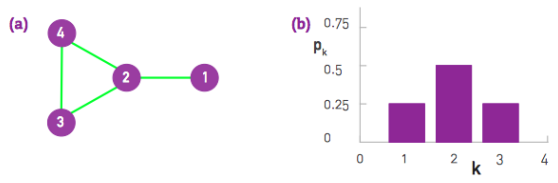
\includegraphics[width=0.7\textwidth]{./img/net/degreedist.png}
    \caption{Esempio di distribuzione dei gradi.}
    \label{fig:degree_distribution}
\end{figure}
\begin{nota}
    Questa distribuzione deve essere normalizzata, ovvero la somma di tutti i
    valori di $p(k)$ deve essere uguale a 1.
    \begin{equation*}
        \sum_{k=0}^{\infty} p(k) = 1
    \end{equation*}
\end{nota}

Il valore della distribuzione mi permette di rappresentare molti fenomeni dalla
robustezza della rete alla sua vulnerabilità.
\subsection{Cammino e distanza}
\begin{definizione}[\textbf{Cammino}]
    Un \textbf{cammino} è una sequenza di nodi in cui ciascun nodo è adiacente
    al successivo.
\end{definizione}
\begin{definizione}[\textbf{Distanza}]
    La \textbf{distanza} tra due nodi è definita come il numero minimo di archi
    che devono essere attraversati per andare da un nodo all'altro. Se i due
    nodi non sono collegati, la distanza è infinita.
\end{definizione}
Un modo semplice per calcolare la distanza tra due nodi è quello di utilizzare
l'algoritmo BFS (Breadth First Search).
\begin{definizione}[\textbf{Diametro}]
    Il diametro di un grafo è la distanza massima tra due nodi nel grafo.
\end{definizione}
\begin{definizione}[\textbf{Lunghezza media dei cammini}]
    La lunghezza media dei cammini è la media delle distanze tra tutti i nodi
    del grafo. Tale misura può essere calcolata come segue:
    \begin{equation}
        \langle d \rangle = \frac{1}{2E_{max}} \sum_{i \neq j} d_{ij}
    \end{equation}
\end{definizione}
Nei grafi non orientati, la lunghezza media dei cammini può essere calcolata
come segue:
\begin{equation}
    \langle d \rangle = \frac{1}{E_{max}} \sum_{i \neq j} d_{ij}
\end{equation}
dove $d_{ij}$ rappresenta la distanza tra i nodi $i$ e $j$ e $E_{max}$ rappresenta
il numero massimo di archi presenti nel grafo.
\subsection{Coefficienti di clustering}
\begin{definizione}[\textbf{Coefficienti di clustering}]
    I coefficienti di clustering sono una misura della presenza di nodi vicini
    tra loro. In particolare, il coefficiente di clustering di un nodo è una
    misura della probabilità che i vicini di un nodo siano collegati tra loro.
    Dato un nodo $i$ con grado $k_i$, il coefficiente di clustering locale è
    definito come segue (grafo indiretto):
    \begin{equation}
        C_i = \frac{2E_i}{k_i(k_i - 1)}
    \end{equation}
    dove $E_i$ rappresenta il numero di archi tra i vicini del nodo $i$. Se il grafo
    è diretto allora si divide per $2$ il coefficiente.
\end{definizione}

Il valore di questo coefficiente può variare tra 0 e 1. Nel caso in cui il
coefficiente sia uguale a 1, significa che tutti i vicini del nodo $i$ sono
collegati tra loro. Nel caso in cui il coefficiente sia uguale a 0, significa
che nessun vicino del nodo $i$ è collegato ad un altro vicino.

Questa misura rappresenta la densità locale di un grafo. Per ottenere una
misura \textbf{globale} della densità del grafo, possiamo calcolare il \textbf{coefficiente
    di clustering medio}. Tale misura può essere calcolata come segue:
\begin{equation}
    \langle C \rangle = \frac{1}{n} \sum_{i=1}^{n} C_i
\end{equation}
dove $\langle C \rangle$ si può interpretare come la probabilità che due vicini
di un nodo, selezionato in modo casuale, siano collegati tra loro.
\begin{definizione}[\textbf{Hub}]
    Un \textbf{hub} è un nodo che ha un grado molto alto, ovvero è connesso a
    molti altri nodi e ha una probabilità molto bassa di occorrere nella rete.
\end{definizione}
\begin{esempio}
    Vediamo ora un esempio di come commentare lo studio di un grafo dal punto di
    vista delle statistiche descrittive. Supponiamo di avere ottenuto un
    i seguenti grafici:
    \begin{figure}[!ht]
        \centering
        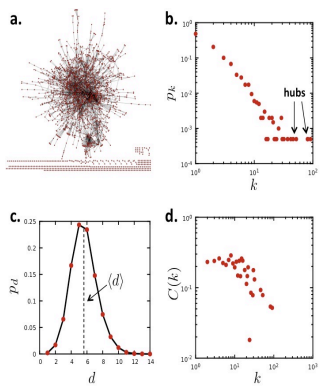
\includegraphics[width=0.7\textwidth]{./img/net/esempio1.png}
        \caption{Esempio di grafici ottenuti dallo studio di un grafo.}
        \label{fig:graphstats}
    \end{figure}

    La distribuzione di grado, riportata nel grafico $b$ della figura \ref{fig:graphstats},
    ci permette di ottenere informazioni in più rispetto alla media. Questo
    perché la media è uno stimatore distorto, sarebbe meglio utilizzare la
    mediana. Inoltre la distribuzione di grado permette di studiare gli \textbf{hub}.

    Il grafico $c$ della figura \ref{fig:graphstats} ci permette di ottenere
    informazioni sul diametro del grafo, sulla lunghezza media dei cammini.

    Il coefficiente di clustering medio permette di capire quanto sono connessi
    i vicini di un nodo estratto casualmente. Il grafico del coefficiente di
    clustering, riportato in figura \ref{fig:graphstats} $d$ mostra le relazioni
    tra grado e clustering. In questo esempio, i nodi spoke hanno un coefficiente
    di clustering maggiore quindi il vicinato è molto connesso, sintomo
    organizzazione gerarchica.

    Con questi ragionamenti si riesce ad effettuare inferenze sul comportamento
    che si ottiene se si dovesse rimuovere un nodo.
\end{esempio}
\section{Centralità del grafo}
La centralità di un nodo è una misura dell'importanza di un nodo all'interno
del grafo. Questa misura può essere calcolata in diversi modi, in base a
diversi criteri. Tra le misure di centralità più comuni troviamo:
\begin{itemize}
    \item \textbf{Degree}
    \item \textbf{Betweeness}
    \item \textbf{Closeness}
    \item \textbf{Autovettori}
    \item \textbf{Pagerank}
\end{itemize}
\begin{definizione}[\textbf{Centralizzazione}]
    La \textbf{centralizzazione} di un grafo è una misura della distribuzione
    della centralità dei nodi del grafo. In particolare, la centralizzazione
    di un grafo è massima quando un nodo ha una centralità molto più alta
    rispetto agli altri nodi del grafo.
\end{definizione}
Il coeff. di centralizzazione: quanta variabilità c'è tra tutte le centralità dei
nodi, è una misura varianza della centralità di grado. Ci serve il coefficiente
di centralità massimo di nodi del grafo ($C_D(n^\ast)$) e la centralizzazione coincide
con la somma degli scarti della centralità tra il nodo con più centralità e tutti gli altri,
infine normalizzo per la massima somma di differenze per una rete che ha $n$ nodi.
Coeff. max ($1$) abbiamo un nodo più centrale rispetto agli altri.

La centralità di grado non è utile per determinare la funzione di ponte (separazione
di gruppi) (è legato la coefficiente di clustering).


\subsection{Degree}
Una delle prime possibilità di misurare la centralità di un nodo è quella di
utilizzare il grado del nodo. Questa misura è particolarmente utile nel caso di
reti sociali, in cui il grado di un nodo corrisponde al numero di amici che
questo nodo ha.
\begin{equation}
    C_D(i) = \sum_{j=1}^{n} x_{ij}
\end{equation}
Nel caso di grafo orientato, possiamo distinguere tra grado entrante e grado
uscente. In particolare, il grado entrante di un nodo corrisponde al numero di
archi che arrivano al nodo, mentre il grado uscente corrisponde al numero di
archi che partono dal nodo.
\begin{equation}
    C_{D_{in}}(i) = \sum_{j=1}^{n} x_{ji} \quad \text{e} \quad
    C_{D_{out}}(i) = \sum_{j=1}^{n} x_{ij}
\end{equation}
La centralità massima per un nodo è $n - 1$.

Questa misura può essere normalizzata ottenendo la centralità di grado normalizzata
dividendo la centralità di grado per il numero di nodi meno uno.

Oltre alla misura di centralità di grado, possiamo calcolare la \textbf{centralizzazione}
di un grafo, ovvero la misura di quanto sia centrale un nodo rispetto agli altri.

La centralizzazione di un grafo può essere calcolata come usando la formula di Freeman:
\begin{equation}
    C_D = \frac{\sum_{i=1}^{n} C_D(n^\ast) - C_D(i)}{(n - 1)(n - 2)}
\end{equation}
dove:
\begin{itemize}
    \item $C_D(n^\ast)$: corrisponde alla centralità massima di un nodo del grafo.
    \item $C_D(i)$: corrisponde alla centralità del nodo $i$.
    \item $n$: corrisponde al numero di nodi del grafo.
\end{itemize}
\subsection{Betweenness}
Un altra misura di centralità è la \textbf{betweeness}, ovvero il nodi più
rilevanti sono quelli che fanno da ponte tra due gruppi di nodi. Posso anche
vederli come nodi che fanno da collo di bottiglia. La betweeness di un nodo
può essere calcolata come segue:
\begin{equation}
    C_B(i) = \sum_{i \neq j \neq k} \frac{g_{jk}(i)}{g_{jk}}
\end{equation}
dove:
\begin{itemize}
    \item $g_{ik}(i)$: corrisponde al numero di \textit{shortest path} tra i
          nodi $j$ e $k$ nella rete tale che il cammino passa per il nodo $i$.
    \item $g_{ik}$: corrisponde al numero di \textit{shortest path} tra i nodi
          $j$ e $k$.
\end{itemize}
In questo caso, la centralità è massima se un nodo ha alta capacità di unire
gruppi. Mentre la centralità tende a $0$ il nodo non collega nessuno.

Viene successivamente fatta una seconda normalizzazione, questa volta sui nodi,
per rendere indipendentemente dalla dimensione del grafo. Questo può essere
espresso nel caso di un grafo non orientato come segue:
\begin{equation}
    C_B(i) = \frac{C_B(i)}{(n - 1)(n - 2)}
\end{equation}
mentre nel caso di un grafo orientato come segue:
\begin{equation}
    C_B(i) = \frac{C_B(i)}{(n - 1)(n - 2) / 2}
\end{equation}
\subsection{Closeness}
La centralità misurata come \textbf{closeness} è una misura della vicinanza di
un nodo agli altri nodi del grafo. Questa misura può essere calcolata come segue:
\begin{equation}
    C_C(i) = \frac{1}{\sum_{j=1}^{n} d_{ij}}
\end{equation}
Corrisponde alla misura di un vertice in merito alla sua efficienza nel
comunicare l'informazione, mentre la betweeness è una misura l'efficacia di un
nodo nell trasmettere un'informazione.

Questa misura può essere normalizzata come segue:
\begin{equation}
    C_C(i) = \frac{C_C(i)}{n - 1}
\end{equation}
\subsection{Autovettori}
La misura dic centralità calcolata utilizzando il grado del nodo rappresenta una
misura locale del grafo. Inoltre, questa misura non tiene conto del ruolo dei
nodi con cui il nodo è collegato. Per ottenere una misura globale della
centralità del nodo, possiamo utilizzare la \textbf{centralità di autovettori}.

La centralità di autovettori è una misura della centralità di un nodo in base
al ruolo dei nodi con cui è collegato, ovvero un nodo è importante se è
collegato ad altri nodi importanti.

Questa misura può essere calcolata come segue:
\begin{equation}
    C_A(i) = \frac{1}{\lambda} \sum_{j=1}^{n} A_{ij} C_A(j)
\end{equation}
dove $A$ è la matrice di adiacenza del grafo e $\lambda$ è l'autovalore
corrispondente all'autovettore dominante della matrice di adiacenza.

A differenza della misura basata sul grado, un nodo che ha un alto grado ma è
collegato a nodi poco importanti avrà una centralità di autovettori bassa. Al
contrario, un nodo che ha un grado basso ma è collegato a nodi molto importanti
avrà una centralità di autovettori alta.
\subsection{Pagerank}
La centralità basata su \textbf{pagerank} è una specializzazione della centralità
di autovettori. Nello specifico questa misura è stata sviluppata per misurare
la centralità di un grafo orientato.

L'assunzione su cui si basa questa misura è che un arco tra il nodo $i$ e il
nodo $j$ rappresenta un voto del nodo $i$ al nodo $j$. Se i due nodi sono connessi
attraverso un arco, la probabilità che i due nodi siano in qualche modo collegati
è maggiore.

L'idea alla base di questa misura è che un nodo $i$ è influenzato dall'importanza
dai nodi che si collegano a lui, in altre parole, gli altri nodi votano per il
nodo $i$.

Il coefficiente di PageRank associato a un nodo $i$ può essere calcolato come:
\begin{equation}
    P(i) = \sum_{(j, i) \in E} \frac{P(j)}{O_j}
\end{equation}
dove $O_j$ rappresenta il numero di archi uscenti dal nodo $j$ e $P$ rappresenta
il vettore di PageRank.

Il vettore di PageRank può essere calcolato andando a risolvere un sistema
lineare di $n$ equazioni in $n$ variabili. In particolare, possiamo scrivere il
vettore di PageRank $P = (P(1), \dots, P(n))^T$ come segue:
\begin{equation}
    P = A^T \cdot P
\end{equation}
dove $A$ è la matrice di adiacenza del grafo definita come:
\begin{equation*}
    A_{ij} = \begin{cases}
        \frac{1}{O_j} & \text{se esiste un arco da $j$ a $i$} \\
        0             & \text{altrimenti}
    \end{cases}
\end{equation*}
A questo punto, la soluzione del problema può essere ottenuta utilizzando un
algoritmo iterativo che restituisce gli autovettori della matrice di adiacenza
normalizzata.

Il problema è che per garantire la convergenza di questo algoritmo è necessario
rispettare due condizioni:
\begin{itemize}
    \item Si ha un unico autovettore dominante.
    \item $P$ è il principale autovettore di $A$.
\end{itemize}

Un'altro possibile metodo per risolvere questo problema è quello di utilizzare
la \textbf{Markov Chain}. In questo caso ogni nodo rappresenta uno stato della
catena e ogni arco rappresenta una transizione che permette di passare da uno
stato all'altro con una certa probabilità.

Questa soluzione permette di simulare la navigazione dell'utente nel web
attraverso diverse pagine e di calcolare la probabilità che l'utente raggiunga
un nodo partendo da un altro nodo.

Per questa soluzione viene utilizzata la matrice di transizione di probabilità
$A$ definita in precedenza, dove ogni elemento $A_{ij}$ rappresenta la probabilità
che l'utente passi dal nodo $i$ al nodo $j$.

A questo punto, partendo da una probabilità iniziale $P_0 = (P_0(1), \dots, P_0(n))^T$
e la matrice di transizione $A$ abbiamo:
\begin{equation*}
    \sum_{i = 1}^n P_0(i) = 1
\end{equation*}
Inoltre, se la matrice $A$ soddisfa la seguente proprietà:
\begin{equation*}
    \sum_{j = 1}^n A_{ij} = 1
\end{equation*}
allora la matrice $A$ è stocastica.

Dal teorema della Markov Chain sappiamo che se la catena di Markov è definita da
una matrice di transizione stocastica allora è caratterizzata da un unica
distribuzione di probabilità stazionaria se $A$ è irriducibile e aperiodica.
\begin{nota}
    Una distribuzione di probabilità stazionaria garantisce che dopo un certo
    numero di passi la probabilità di raggiungere un nodo da tutti gli altri
    nodi non cambia.
\end{nota}
Per garantire questo devono essere verificate le seguenti condizioni:
\begin{itemize}
    \item La matrice $A$ deve essere stocastica, ovvero la somma di ogni riga
          deve essere uguale a 1.
          \begin{equation*}
              \sum_{j = 1}^n A_{ij} = 1
          \end{equation*}
          Un problema in questo caso è rappresentato da una pagina che non ha
          link uscenti, essa sarebbe rappresentata da una riga di $0$. Si hanno
          due possibili soluzioni:
          \begin{itemize}
              \item Aggiungere un arco uscente per ogni nodo che non rispetta la
                    condizione.
              \item Rimuovere tutte le pagine che non hanno link uscenti.
          \end{itemize}
    \item \textbf{Irriducibilità}: se il grafo è fortemente connesso.
    \item \textbf{Aperiodicità}: se tutti gli stati della catena sono aperiodici,
          ovvero se non fa parte di cicli.
\end{itemize}
Una soluzione alle problematiche relative alla irriducibilità e aperiodicità
si ottiene aggiungendo un arco da ogni nodo a tutti gli altri nodi del grafo con
una probabilità di transizione molto bassa controllata da un parametro $d$:
\begin{equation}
    A_{ij} = (1 - d) + d \cdot \sum_{(j, i) \in E}\frac{P(j)}{O_j}
\end{equation}

Il coefficiente di PageRank $P_i$ può essere calcolato risolvendo il seguente
sistema di equazioni:
\begin{equation}
    \left[
        \begin{array}{c}
            P_1    \\
            \vdots \\
            P_n
        \end{array}
        \right] = d \cdot \left[
        \begin{array}{ccc}
            A_{11} & \dots  & A_{1, n} \\
            \vdots & \ddots & \vdots   \\
            A_{n1} & \dots  & A_{nn}
        \end{array}
        \right] + (1 - d) \cdot \left[
        \begin{array}{c}
            1      \\
            \vdots \\
            1
        \end{array} \right]
\end{equation}
Sotto la seguente condizione:
\begin{equation*}
    \sum_{i}^n P_i = 1
\end{equation*}
